\documentclass[conference]{IEEEtran}
\usepackage{graphicx}
\usepackage{booktabs}
\usepackage{amsmath,amssymb}
\usepackage{url}
\usepackage[hidelinks]{hyperref}
\usepackage{xcolor}
\usepackage{siunitx}
\graphicspath{{../experiments/ndws/}}

% All result numbers are generated by `python -m src.aml.evaluate`.
% Generated by `python -m src.aml.evaluate`. Do not edit by hand.
\newcommand{\OfficialPersistencePR}{0.107}
\newcommand{\OfficialPersistencePRlo}{0.097}
\newcommand{\OfficialPersistencePRhi}{0.118}
\newcommand{\OfficialPersistenceLift}{8.5}
\newcommand{\OfficialPersistenceROC}{0.633}
\newcommand{\OfficialPersistenceFone}{0.309}
\newcommand{\OfficialPersistencePrec}{0.357}
\newcommand{\OfficialPersistenceRec}{0.273}
\newcommand{\OfficialPersistenceRone}{0.276}
\newcommand{\OfficialPersistenceRfive}{0.305}
\newcommand{\OfficialPersistenceBrier}{0.0153}
\newcommand{\OfficialPersistenceValPR}{0.060}
\newcommand{\OfficialNbrPersistPR}{0.173}
\newcommand{\OfficialNbrPersistPRlo}{0.157}
\newcommand{\OfficialNbrPersistPRhi}{0.191}
\newcommand{\OfficialNbrPersistLift}{13.8}
\newcommand{\OfficialNbrPersistROC}{0.729}
\newcommand{\OfficialNbrPersistFone}{0.337}
\newcommand{\OfficialNbrPersistPrec}{0.288}
\newcommand{\OfficialNbrPersistRec}{0.407}
\newcommand{\OfficialNbrPersistRone}{0.360}
\newcommand{\OfficialNbrPersistRfive}{0.491}
\newcommand{\OfficialNbrPersistBrier}{0.0121}
\newcommand{\OfficialNbrPersistValPR}{0.094}
\newcommand{\OfficialLogRegPR}{0.230}
\newcommand{\OfficialLogRegPRlo}{0.213}
\newcommand{\OfficialLogRegPRhi}{0.249}
\newcommand{\OfficialLogRegLift}{18.4}
\newcommand{\OfficialLogRegROC}{0.903}
\newcommand{\OfficialLogRegFone}{0.327}
\newcommand{\OfficialLogRegPrec}{0.246}
\newcommand{\OfficialLogRegRec}{0.488}
\newcommand{\OfficialLogRegRone}{0.363}
\newcommand{\OfficialLogRegRfive}{0.665}
\newcommand{\OfficialLogRegBrier}{0.0106}
\newcommand{\OfficialLogRegValPR}{0.158}
\newcommand{\OfficialRandomForestPR}{0.265}
\newcommand{\OfficialRandomForestPRlo}{0.248}
\newcommand{\OfficialRandomForestPRhi}{0.282}
\newcommand{\OfficialRandomForestLift}{21.1}
\newcommand{\OfficialRandomForestROC}{0.901}
\newcommand{\OfficialRandomForestFone}{0.343}
\newcommand{\OfficialRandomForestPrec}{0.261}
\newcommand{\OfficialRandomForestRec}{0.498}
\newcommand{\OfficialRandomForestRone}{0.389}
\newcommand{\OfficialRandomForestRfive}{0.679}
\newcommand{\OfficialRandomForestBrier}{0.0104}
\newcommand{\OfficialRandomForestValPR}{0.205}
\newcommand{\OfficialXGBoostPR}{0.265}
\newcommand{\OfficialXGBoostPRlo}{0.248}
\newcommand{\OfficialXGBoostPRhi}{0.283}
\newcommand{\OfficialXGBoostLift}{21.1}
\newcommand{\OfficialXGBoostROC}{0.911}
\newcommand{\OfficialXGBoostFone}{0.332}
\newcommand{\OfficialXGBoostPrec}{0.242}
\newcommand{\OfficialXGBoostRec}{0.528}
\newcommand{\OfficialXGBoostRone}{0.389}
\newcommand{\OfficialXGBoostRfive}{0.680}
\newcommand{\OfficialXGBoostBrier}{0.0104}
\newcommand{\OfficialXGBoostValPR}{0.206}
\newcommand{\OfficialLightGBMPR}{0.263}
\newcommand{\OfficialLightGBMPRlo}{0.246}
\newcommand{\OfficialLightGBMPRhi}{0.281}
\newcommand{\OfficialLightGBMLift}{20.9}
\newcommand{\OfficialLightGBMROC}{0.905}
\newcommand{\OfficialLightGBMFone}{0.334}
\newcommand{\OfficialLightGBMPrec}{0.245}
\newcommand{\OfficialLightGBMRec}{0.525}
\newcommand{\OfficialLightGBMRone}{0.387}
\newcommand{\OfficialLightGBMRfive}{0.680}
\newcommand{\OfficialLightGBMBrier}{0.0104}
\newcommand{\OfficialLightGBMValPR}{0.204}
\newcommand{\OfficialPosRate}{1.25\%}
\newcommand{\OfficialPixels}{6{,}727{,}699}
\newcommand{\OfficialDeltaLightGBMvsLogReg}{+0.032~[+0.025, +0.040]}
\newcommand{\OfficialDeltaLightGBMvsRandomForest}{-0.002~[-0.008, +0.003]}
\newcommand{\OfficialDeltaLightGBMvsXGBoost}{-0.002~[-0.006, +0.001]}
\newcommand{\OfficialDeltaLightGBMvsPersistence}{+0.156~[+0.147, +0.165]}
\newcommand{\OfficialDeltaXGBoostvsLogReg}{+0.035~[+0.028, +0.042]}
\newcommand{\OfficialDeltaLogRegvsPersistence}{+0.124~[+0.115, +0.132]}
\newcommand{\OfficialResultsTable}{%
Persistence & 0.107 [0.097, 0.118] & 8.5$\times$ & 0.633 & 0.309 & 0.276 & 0.305 & 0.0153 \\
Neighbourhood persistence & 0.173 [0.157, 0.191] & 13.8$\times$ & 0.729 & 0.337 & 0.360 & 0.491 & 0.0121 \\
Logistic regression & 0.230 [0.213, 0.249] & 18.4$\times$ & 0.903 & 0.327 & 0.363 & 0.665 & 0.0106 \\
Random forest & 0.265 [0.248, 0.282] & 21.1$\times$ & 0.901 & 0.343 & 0.389 & 0.679 & 0.0104 \\
XGBoost & 0.265 [0.248, 0.283] & 21.1$\times$ & 0.911 & 0.332 & 0.389 & 0.680 & 0.0104 \\
LightGBM & 0.263 [0.246, 0.281] & 20.9$\times$ & 0.905 & 0.334 & 0.387 & 0.680 & 0.0104 \\
}
\newcommand{\SpatialPersistencePR}{0.037}
\newcommand{\SpatialPersistencePRlo}{0.032}
\newcommand{\SpatialPersistencePRhi}{0.041}
\newcommand{\SpatialPersistenceLift}{7.6}
\newcommand{\SpatialPersistenceROC}{0.572}
\newcommand{\SpatialPersistenceFone}{0.177}
\newcommand{\SpatialPersistencePrec}{0.224}
\newcommand{\SpatialPersistenceRec}{0.146}
\newcommand{\SpatialPersistenceRone}{0.152}
\newcommand{\SpatialPersistenceRfive}{0.186}
\newcommand{\SpatialPersistenceBrier}{0.0066}
\newcommand{\SpatialPersistenceValPR}{0.070}
\newcommand{\SpatialNbrPersistPR}{0.064}
\newcommand{\SpatialNbrPersistPRlo}{0.055}
\newcommand{\SpatialNbrPersistPRhi}{0.071}
\newcommand{\SpatialNbrPersistLift}{13.2}
\newcommand{\SpatialNbrPersistROC}{0.641}
\newcommand{\SpatialNbrPersistFone}{0.203}
\newcommand{\SpatialNbrPersistPrec}{0.181}
\newcommand{\SpatialNbrPersistRec}{0.230}
\newcommand{\SpatialNbrPersistRone}{0.292}
\newcommand{\SpatialNbrPersistRfive}{0.320}
\newcommand{\SpatialNbrPersistBrier}{0.0053}
\newcommand{\SpatialNbrPersistValPR}{0.118}
\newcommand{\SpatialLogRegPR}{0.117}
\newcommand{\SpatialLogRegPRlo}{0.106}
\newcommand{\SpatialLogRegPRhi}{0.127}
\newcommand{\SpatialLogRegLift}{24.2}
\newcommand{\SpatialLogRegROC}{0.867}
\newcommand{\SpatialLogRegFone}{0.226}
\newcommand{\SpatialLogRegPrec}{0.193}
\newcommand{\SpatialLogRegRec}{0.272}
\newcommand{\SpatialLogRegRone}{0.374}
\newcommand{\SpatialLogRegRfive}{0.639}
\newcommand{\SpatialLogRegBrier}{0.0045}
\newcommand{\SpatialLogRegValPR}{0.188}
\newcommand{\SpatialRandomForestPR}{0.135}
\newcommand{\SpatialRandomForestPRlo}{0.123}
\newcommand{\SpatialRandomForestPRhi}{0.149}
\newcommand{\SpatialRandomForestLift}{28.1}
\newcommand{\SpatialRandomForestROC}{0.885}
\newcommand{\SpatialRandomForestFone}{0.234}
\newcommand{\SpatialRandomForestPrec}{0.191}
\newcommand{\SpatialRandomForestRec}{0.304}
\newcommand{\SpatialRandomForestRone}{0.382}
\newcommand{\SpatialRandomForestRfive}{0.627}
\newcommand{\SpatialRandomForestBrier}{0.0044}
\newcommand{\SpatialRandomForestValPR}{0.228}
\newcommand{\SpatialXGBoostPR}{0.141}
\newcommand{\SpatialXGBoostPRlo}{0.128}
\newcommand{\SpatialXGBoostPRhi}{0.154}
\newcommand{\SpatialXGBoostLift}{29.1}
\newcommand{\SpatialXGBoostROC}{0.899}
\newcommand{\SpatialXGBoostFone}{0.246}
\newcommand{\SpatialXGBoostPrec}{0.230}
\newcommand{\SpatialXGBoostRec}{0.263}
\newcommand{\SpatialXGBoostRone}{0.382}
\newcommand{\SpatialXGBoostRfive}{0.628}
\newcommand{\SpatialXGBoostBrier}{0.0044}
\newcommand{\SpatialXGBoostValPR}{0.230}
\newcommand{\SpatialLightGBMPR}{0.138}
\newcommand{\SpatialLightGBMPRlo}{0.127}
\newcommand{\SpatialLightGBMPRhi}{0.150}
\newcommand{\SpatialLightGBMLift}{28.6}
\newcommand{\SpatialLightGBMROC}{0.896}
\newcommand{\SpatialLightGBMFone}{0.244}
\newcommand{\SpatialLightGBMPrec}{0.229}
\newcommand{\SpatialLightGBMRec}{0.261}
\newcommand{\SpatialLightGBMRone}{0.382}
\newcommand{\SpatialLightGBMRfive}{0.621}
\newcommand{\SpatialLightGBMBrier}{0.0044}
\newcommand{\SpatialLightGBMValPR}{0.230}
\newcommand{\SpatialPosRate}{0.48\%}
\newcommand{\SpatialPixels}{7{,}199{,}385}
\newcommand{\SpatialDeltaLightGBMvsLogReg}{+0.021~[+0.016, +0.026]}
\newcommand{\SpatialDeltaLightGBMvsRandomForest}{+0.003~[-0.002, +0.006]}
\newcommand{\SpatialDeltaLightGBMvsXGBoost}{-0.002~[-0.007, +0.001]}
\newcommand{\SpatialDeltaLightGBMvsPersistence}{+0.101~[+0.093, +0.110]}
\newcommand{\SpatialDeltaXGBoostvsLogReg}{+0.024~[+0.018, +0.030]}
\newcommand{\SpatialDeltaLogRegvsPersistence}{+0.080~[+0.072, +0.088]}
\newcommand{\SpatialResultsTable}{%
Persistence & 0.037 [0.032, 0.041] & 7.6$\times$ & 0.572 & 0.177 & 0.152 & 0.186 & 0.0066 \\
Neighbourhood persistence & 0.064 [0.055, 0.071] & 13.2$\times$ & 0.641 & 0.203 & 0.292 & 0.320 & 0.0053 \\
Logistic regression & 0.117 [0.106, 0.127] & 24.2$\times$ & 0.867 & 0.226 & 0.374 & 0.639 & 0.0045 \\
Random forest & 0.135 [0.123, 0.149] & 28.1$\times$ & 0.885 & 0.234 & 0.382 & 0.627 & 0.0044 \\
XGBoost & 0.141 [0.128, 0.154] & 29.1$\times$ & 0.899 & 0.246 & 0.382 & 0.628 & 0.0044 \\
LightGBM & 0.138 [0.127, 0.150] & 28.6$\times$ & 0.896 & 0.244 & 0.382 & 0.621 & 0.0044 \\
}
\newcommand{\SpatialAblationTable}{%
\texttt{raw\_only} & 10 & 0.025 & 0.010 \\
\texttt{fire\_only} & 8 & 0.191 & 0.111 \\
\texttt{raw+fire} & 18 & 0.212 & 0.130 \\
\texttt{raw+fire+wind} & 24 & 0.226 & 0.140 \\
\texttt{raw+fire+wind+terrain} & 28 & 0.228 & 0.142 \\
\texttt{all\_features} & 32 & 0.230 & 0.138 \\
\texttt{all\_minus\_raw} & 22 & 0.226 & 0.138 \\
\texttt{all\_minus\_fire} & 24 & 0.213 & 0.131 \\
\texttt{all\_minus\_wind} & 26 & 0.220 & 0.139 \\
\texttt{all\_minus\_terrain} & 28 & 0.227 & 0.139 \\
\texttt{all\_minus\_weather} & 30 & 0.227 & 0.141 \\
\texttt{all\_minus\_vegetation} & 30 & 0.227 & 0.146 \\
}


\begin{document}

\title{Next-Day Wildfire Spread Prediction with Engineered Tabular Features:\\
A Leakage-Aware Evaluation on the NDWS Benchmark}

\author{
\IEEEauthorblockN{Vedant Satbhai, Pratik Agade, Lakshay Saharan, Raghvendra Singh, Aaryan Krishna}
\IEEEauthorblockA{CSAI, Newton School of Technology, Rishihood University\\
\{vedant.satbhai2024, pratik.agade2024, lakshay.saharan2024, raghvendra.singh2024, aaryan.krishna2024\}@nst.rishihood.edu.in\\
Project 17 --- Phase 1 (Machine Learning)}
}

\maketitle

\begin{abstract}
We predict, for every \SI{1}{km} pixel of a region with an active fire, whether it burns the next day, using the
Next Day Wildfire Spread (NDWS) dataset. Each pixel is described by 32 engineered features: lagged burn activity at
four spatial scales, distance to the fire front, wind--fire alignment, terrain relative to the fire, dryness indicators
and local vegetation statistics. We compare persistence baselines, logistic regression, random forest, XGBoost and
LightGBM. On the official split, XGBoost reaches PR-AUC \OfficialXGBoostPR{} (95\% CI
\OfficialXGBoostPRlo--\OfficialXGBoostPRhi), above the 0.198 and 0.225 reported for the dataset paper's logistic
regression and random forest baselines and close to its convolutional model (0.284). Using a terrain fingerprint, we
find that about 95\% of official test patches cover the same ground as training patches. We therefore also evaluate on a
location-grouped split with no shared terrain, where XGBoost reaches \SpatialXGBoostPR{}
(\SpatialXGBoostLift$\times$ chance). Gradient boosting beats logistic regression significantly on both protocols but is
statistically tied with a random forest. Despite the overlap, prevalence-normalised performance and model ranking barely
change between protocols. The large drop in raw PR-AUC reflects the smaller, rarer fires in the held-out location
groups. Ablations show that lagged burn features carry most of the signal and wind adds a smaller gain. These results
leave room for the spatial deep models of Phase~2.
\end{abstract}

\begin{IEEEkeywords}
wildfire spread, gradient boosting, remote sensing, spatial leakage, imbalanced classification
\end{IEEEkeywords}

% -------------------------------------------------------------------------
\section{Introduction}
Wildfire agencies need to know where a fire will be tomorrow in order to place crews, issue evacuations and plan
containment lines. Physics-based simulators such as FARSITE~\cite{finney1998farsite}, built on Rothermel's spread
model~\cite{rothermel1972}, need detailed fuel and wind inputs and are expensive to run as ensembles. The NDWS
dataset~\cite{huot2022ndws} instead frames next-day spread as per-pixel segmentation from remote-sensing, weather
and terrain rasters.

The project brief asks for a strong tabular baseline (XGBoost or LightGBM on engineered features) before spatial deep
learning, and for evaluation that separates events spatially and temporally and reports PR-AUC, recall at fixed false
positive rate, F1 and ROC-AUC. Our contributions are:
\begin{enumerate}
\item A 32-feature, physically motivated tabular representation of each pixel, with every feature computed only from
day-$t$ inputs.
\item A \emph{terrain-fingerprint} leakage audit showing that the official NDWS split shares terrain between train and
test for about 95\% of test patches, and a location-grouped split that removes this overlap.
\item A tuned comparison of five learners plus two baselines, with patch-bootstrap confidence intervals, paired
significance tests, feature-group ablations, SHAP attributions and physical-plausibility checks.
\end{enumerate}

% -------------------------------------------------------------------------
\section{Related Work}
Jain \textit{et al.}~\cite{jain2020review} review machine learning in wildfire science and note the lack of shared
benchmarks. CNN spread models~\cite{radke2019firecast,hodges2019cnn} and remote-sensing occurrence
datasets~\cite{sayad2019predictive} each used their own data. NDWS~\cite{huot2022ndws} provides 18{,}545 samples
(US, 2012--2020) with an official split by random weeks. Its pixel-level baselines (pixel plus 3$\times$3 neighbours)
reach PR-AUC 0.198 (logistic regression) and 0.225 (random forest), against 0.115 for persistence and 0.284 for a
convolutional autoencoder. WildfireSpreadTS~\cite{gerard2023wildfirespreadts} adds multi-day sequences with event
identifiers. Our learners are random forests~\cite{breiman2001rf} and gradient boosting~\cite{friedman2001gbm} in the
XGBoost~\cite{chen2016xgboost} and LightGBM~\cite{ke2017lightgbm} implementations, with SHAP
attributions~\cite{lundberg2017shap}. Our evaluation follows advice on PR analysis under
imbalance~\cite{saito2015pr}, grouped cross-validation for spatially structured data~\cite{roberts2017cv}, calibration
of tree ensembles~\cite{niculescu2005calibration}, and prior correction after class
resampling~\cite{saerens2002prior}.

% -------------------------------------------------------------------------
\section{Data and Exploratory Analysis}
\subsection{Dataset}
Each NDWS sample is a 64$\times$64 grid of \SI{1}{km} pixels with 11 inputs: elevation (SRTM); wind direction and
speed, minimum and maximum temperature, specific humidity, precipitation and drought index (GRIDMET~\cite{abatzoglou2013gridmet});
NDVI (VIIRS); population density; and the energy release component (ERC). It also contains the day-$t$ MODIS fire mask.
The target is the day-$t{+}1$ fire mask. Masks take values 1 (fire), 0 (no fire) and $-1$ (unknown, e.g.\ cloud).
The official split has 14{,}979 / 1{,}877 / 1{,}689 patches.

\subsection{Class balance and label noise}
About 1.1\% of known-label pixels are positive, and 2.4\% of target pixels are unknown (excluded throughout). Only
about 26\% of next-day fire pixels were already burning on day $t$, so copying the current mask (persistence) misses
most of the target (Fig.~\ref{fig:eda}a). New fire concentrates within a few kilometres of the day-$t$ fire: about 20\%
of non-burning pixels within \SI{1.5}{km} ignite, against 0.4\% at 10--\SI{15}{km}.

\subsection{Data quality}
The audit found physically impossible values. Temperatures of 0~K (missing values) and up to 344~K (71\,$^\circ$C)
occur, as do negative humidity and wind speed, and corrupted wind directions (down to $-4.97\times10^5$ degrees in about
0.2\% of pixels). Values outside physical ranges are set to missing. Negative precipitation is clipped. NDVI is
rescaled to $[-1,1]$ and population log-transformed. Sub-sea-level elevations are kept.

\subsection{Orientation as a physical test}
The Kaggle release carries no georeferencing, so we tested all four row/column conventions. We compare the probability
that a non-burning pixel ignites when day-$t$ fire lies 1--\SI{3}{km} upwind of it with the probability when fire lies
downwind of it. Only rows running south$\rightarrow$north with columns west$\rightarrow$east gives a ratio significantly
above one: 1.12 (95\% patch-bootstrap CI 1.09--1.15), against 1.01 (0.98--1.04) for the opposite row order. We adopt
that convention. Within \SI{3}{km} of fire, sloped pixels (up- or downslope) ignite about twice as often as level ones.

\begin{figure}[t]
\centering
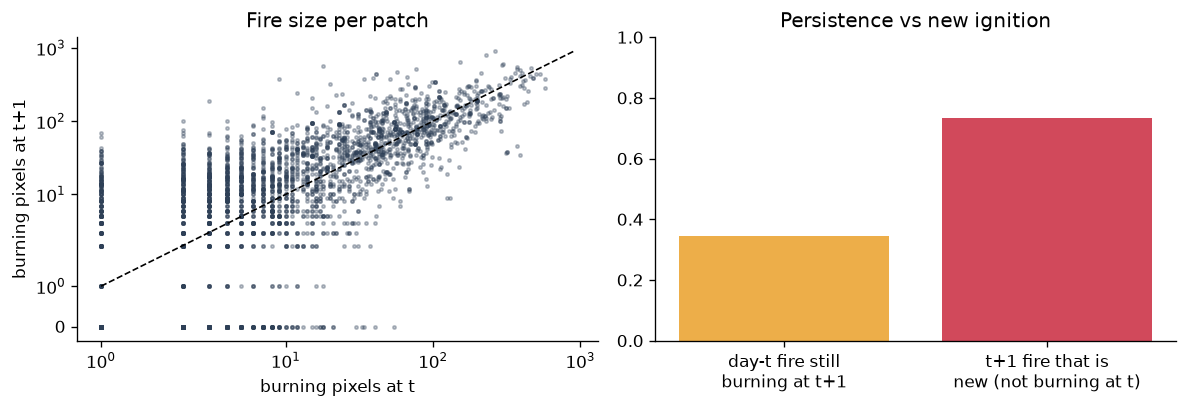
\includegraphics[width=\columnwidth]{eda/fire_dynamics.png}\\[2pt]
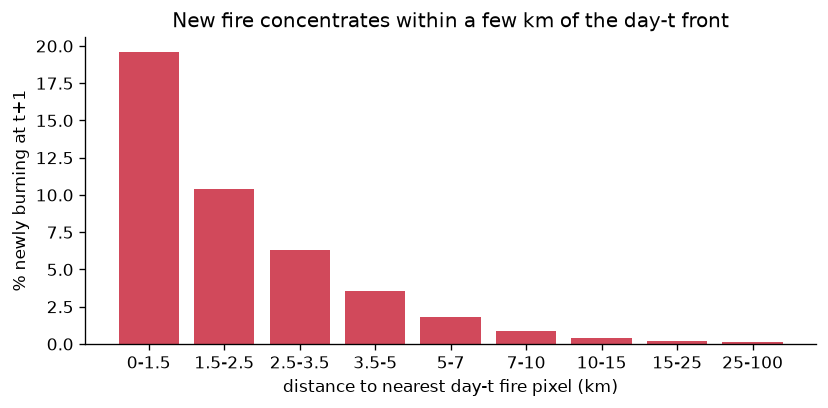
\includegraphics[width=0.49\columnwidth]{eda/spread_vs_distance.png}\hfill
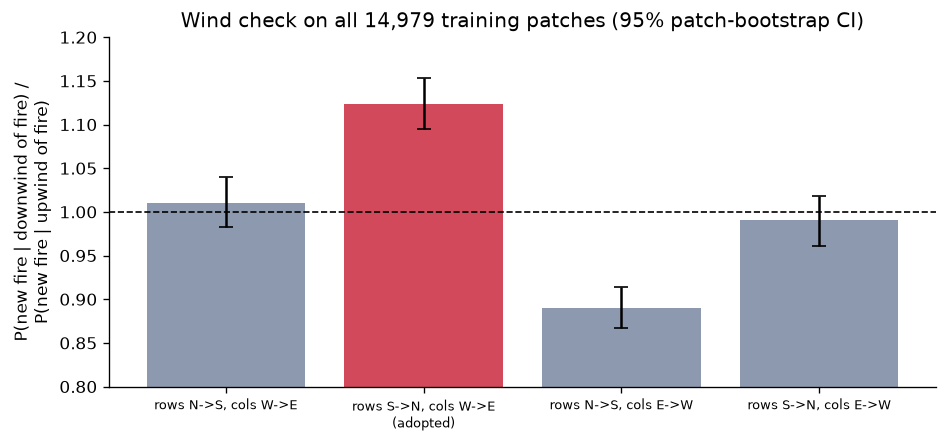
\includegraphics[width=0.49\columnwidth]{eda/wind_orientation.png}
\caption{EDA. (a) Fire size at $t$ vs.\ $t{+}1$ and the share of new fire. (b) Ignition rate vs.\ distance to the
day-$t$ front. (c) Downwind/upwind spread ratio under each orientation convention.}
\label{fig:eda}
\end{figure}

% -------------------------------------------------------------------------
\section{Spatial Leakage Audit and Splits}
Elevation is static, so two patches containing an identical non-flat 8$\times$\SI{8}{km} elevation block
(standard deviation $>\SI{5}{m}$) cover the same ground. We hash every such block on a stride-8 grid. We then slide an
8$\times$8 window over every patch, look up its hash, and join matching patches with union-find. The result is 845
location groups. As a control, horizontally mirrored patches produce 0 matches in 1{,}855 trials. About \textbf{95\% of
official test patches (1{,}606 / 1{,}689) belong to a group that also appears in training}. The official split is
therefore temporally separated (by week) but not spatially.

The \emph{spatial} protocol assigns whole location groups to train / validation / test (14{,}822 / 1{,}855 / 1{,}868
patches), so no held-out patch shares terrain with training. Consecutive days of one fire overlap in terrain and land in
the same group, so the split is also event-disjoint. The two largest groups (7{,}246 and 5{,}952 patches, recurring
fire regions) must stay in training. As a result, the held-out groups contain smaller, more isolated fires: the
spatial test positive rate is \SpatialPosRate{} against \OfficialPosRate{} for the official test. Because PR-AUC's
chance level equals prevalence, we compare protocols through lift (PR-AUC divided by prevalence) and ROC-AUC.

% -------------------------------------------------------------------------
\section{Feature Engineering}
Table~\ref{tab:features} lists the 32 features. Neighbourhood burn fractions use box filters of size 3, 5, 9 and 17;
distance to fire uses a Euclidean distance transform. Wind--fire alignment is the cosine between the wind's
travel direction and the vector from the nearest burning pixel. Vapour-pressure deficit uses the Tetens equation at
$T_{\max}$ and the FAO-56 pressure--elevation relation~\cite{allen1998fao56}: $\mathrm{VPD}=0.6108\,e^{17.27T/(T+237.3)} - qp/(0.622+0.378q)$.
A unit test checks that changing the target mask leaves every feature unchanged.

\begin{table}[t]
\caption{Engineered features (all from day-$t$ inputs)}
\label{tab:features}
\centering\footnotesize
\begin{tabular}{@{}lp{5.6cm}@{}}
\toprule
Group & Features \\
\midrule
raw (10) & elevation, wind speed, $T_{\min}$, $T_{\max}$, humidity, precipitation, PDSI, NDVI, log population, ERC \\
fire (8) & day-$t$ fire, unknown flag, burning fraction in 3/5/9/17\,km windows, distance to fire, log patch fire count \\
wind (6) & $u$, $v$; fire 1--3\,km upwind / downwind; wind--fire alignment; alignment$\times$speed$/(1+d)$ \\
terrain (4) & slope, aspect (sin, cos), rise over run from nearest fire \\
weather (2) & $T_{\max}-T_{\min}$, vapour-pressure deficit \\
vegetation (2) & 5$\times$5 NDVI mean and standard deviation \\
\bottomrule
\end{tabular}
\end{table}

% -------------------------------------------------------------------------
\section{Models and Training}
\subsection{Learners}
\emph{Logistic regression} minimises the L2-regularised log-loss
$-\sum_i[y_i\log p_i+(1-y_i)\log(1-p_i)]+\lambda\|w\|^2$ with $p_i=\sigma(w^\top x_i+b)$, after median imputation and
standardisation. A \emph{random forest} averages decorrelated trees; for $B$ trees with variance $\sigma^2$ and pairwise
correlation $\rho$, the ensemble variance is $\rho\sigma^2+(1-\rho)\sigma^2/B$. \emph{Gradient boosting} adds trees fitted
to the loss gradient. With per-leaf gradient and hessian sums $G,H$ (for log-loss $g=p-y$, $h=p(1-p)$), XGBoost sets
leaf weights $w^\star=-G/(H+\lambda)$ and scores splits by
$\tfrac12\big[\tfrac{G_L^2}{H_L+\lambda}+\tfrac{G_R^2}{H_R+\lambda}-\tfrac{(G_L+G_R)^2}{H_L+H_R+\lambda}\big]-\gamma$.
LightGBM grows trees leaf-wise.

\subsection{Imbalance and calibration}
Training rows are all positive pixels plus a random 2\% of negative pixels from the training split (1.92\,M rows on
the spatial protocol). Validation and test are never resampled. For each learner we either (i) weight negatives by 50,
restoring the true prior, or (ii) train unweighted and map probabilities back with
$p=rp_s/(rp_s+1-p_s)$, $r=0.02$~\cite{saerens2002prior}. The choice is made on validation. Option (ii) is monotone, so
ranking metrics are unaffected.

\subsection{Model selection}
Pixels within a patch share almost constant weather values, so trees with small leaves memorise patches. An initial
LightGBM configuration (minimum leaf 200, importance weights) stopped after five trees. We therefore use minimum leaf
sizes of 2{,}000--5{,}000, column subsampling of 0.5, and early stopping on validation PR-AUC. Small grids (three
LightGBM and two XGBoost configurations) are compared by PR-AUC on all validation pixels. The F1 threshold of each
model is also chosen on validation. The test split is scored once.

% -------------------------------------------------------------------------
\section{Evaluation Protocol}
We report PR-AUC (average precision), lift over chance, ROC-AUC, F1 at the validation-chosen threshold, recall at 1\%
and 5\% false-positive rate, and the Brier score. Accuracy is omitted because predicting ``no fire'' scores about 99\%.
Pixels in a patch are correlated, so 95\% confidence intervals come from a bootstrap over \emph{patches} (500
replicates). Model differences use a paired bootstrap of $\Delta$PR-AUC on the same resamples.

% -------------------------------------------------------------------------
\section{Results}
\begin{table*}[t]
\caption{Test results. PR-AUC with 95\% patch-bootstrap CI; lift = PR-AUC / prevalence; F1 at the validation threshold;
R@1\%/R@5\% = recall at 1\%/5\% FPR.}
\label{tab:results}
\centering\footnotesize
\begin{tabular}{@{}lccccccc@{}}
\toprule
Model & PR-AUC [95\% CI] & Lift & ROC-AUC & F1 & R@1\% & R@5\% & Brier \\
\midrule
\multicolumn{8}{@{}l}{\emph{Spatial protocol (no shared terrain; test prevalence \SpatialPosRate, \SpatialPixels{} pixels)}} \\
\SpatialResultsTable
\midrule
\multicolumn{8}{@{}l}{\emph{Official NDWS protocol (week-separated; test prevalence \OfficialPosRate, \OfficialPixels{} pixels)}} \\
\OfficialResultsTable
\bottomrule
\end{tabular}
\end{table*}

\subsection{Main comparison}
Table~\ref{tab:results} shows that all learned models beat both persistence baselines by a wide margin on both
protocols. Our persistence PR-AUC on the official test (\OfficialPersistencePR) matches the 0.115 reported by Huot
\textit{et al.}, which supports the comparability of our evaluation. With engineered features, our logistic regression
(\OfficialLogRegPR) and random forest (\OfficialRandomForestPR) exceed their published counterparts (0.198, 0.225), and
gradient boosting reaches \OfficialXGBoostPR{}, close to their convolutional autoencoder (0.284).

Paired bootstrap differences (95\% CI) show where the gains are robust. LightGBM beats logistic regression on both
protocols (spatial \SpatialDeltaLightGBMvsLogReg; official \OfficialDeltaLightGBMvsLogReg). It does \emph{not}
significantly beat the random forest (spatial \SpatialDeltaLightGBMvsRandomForest; official
\OfficialDeltaLightGBMvsRandomForest), and LightGBM and XGBoost are tied (\SpatialDeltaLightGBMvsXGBoost). Non-linear
interactions matter, but on these features the choice among tree ensembles does not. Boosted models are also the best
calibrated (Brier \SpatialLightGBMBrier, Fig.~\ref{fig:pr} and repository reliability plots).

\subsection{Effect of spatial overlap}
Raw PR-AUC roughly halves on the spatial test, but test prevalence also falls from \OfficialPosRate{} to
\SpatialPosRate. Prevalence-independent measures tell a different story. LightGBM's ROC-AUC changes only from
\OfficialLightGBMROC{} to \SpatialLightGBMROC, its lift is actually higher on the spatial test
(\SpatialLightGBMLift$\times$ vs.\ \OfficialLightGBMLift$\times$), and the ranking of all six methods is identical. We
therefore find no evidence that the terrain overlap substantially inflates the official benchmark for pixel-level
tabular models. One sign of mild location memorisation remains: static location fields (elevation, population) carry
more SHAP weight under the official protocol than under the spatial one. The validation PR-AUC on the spatial protocol
(\SpatialLightGBMValPR) is also well above its test value, so held-out location groups differ substantially from each
other. Single-split NDWS numbers should be read with their intervals and prevalence.

\begin{figure}[t]
\centering
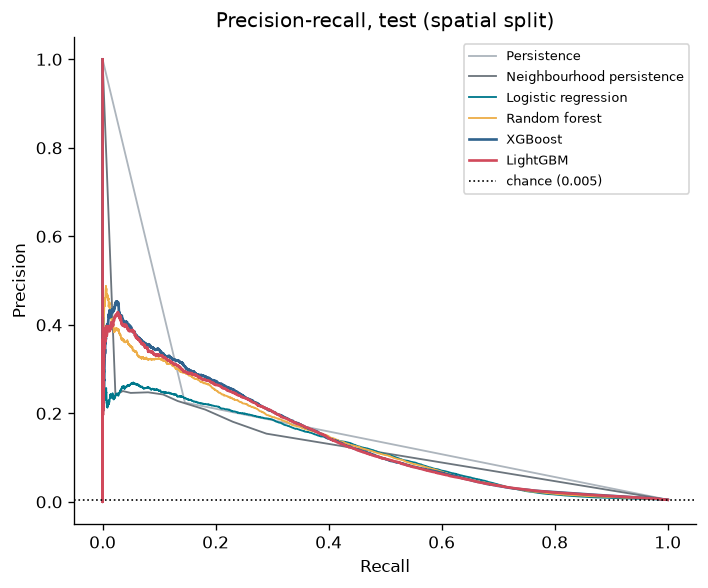
\includegraphics[width=\columnwidth]{results/spatial/pr_curves.png}
\caption{Precision--recall curves on the spatial test split. Chance level is the prevalence (\SpatialPosRate).}
\label{fig:pr}
\end{figure}

\subsection{Ablation}
Table~\ref{tab:ablation} retrains the selected LightGBM configuration on subsets of feature groups. Raw environmental
channels alone are barely above chance: they describe conditions that are almost constant across a patch, not where
fire will appear. Lagged burn features alone recover most of the performance, and removing them causes the largest
drop. Adding wind features to raw+fire gives the next-largest gain on both validation and test. Terrain, dryness and
vegetation change test PR-AUC by less than the bootstrap uncertainty (about $\pm0.01$), so we do not claim they help.

\begin{table}[t]
\caption{LightGBM feature-group ablation (spatial protocol, PR-AUC)}
\label{tab:ablation}
\centering\footnotesize
\begin{tabular}{@{}lccc@{}}
\toprule
Feature set & \# & Val & Test \\
\midrule
\SpatialAblationTable
\bottomrule
\end{tabular}
\end{table}

\subsection{Interpretation and plausibility}
SHAP values (Fig.~\ref{fig:shap}) rank distance to fire and the 17, 9 and 5\,km burn fractions highest, followed by
wind push (positive when the pixel lies downwind of fire), relative elevation to the fire, and NDVI. High VPD raises
predicted risk, as dryness physics suggests. In the plausibility checks, mean predicted probability tracks the observed
ignition rate across distance bins (e.g.\ 0.124 predicted vs.\ 0.117 observed within 1.5\,km on the spatial test). It
also rises from upwind to downwind pixels as the observed rate does, and is higher on sloped than level ground near fire.
Probability maps (Fig.~\ref{fig:maps}) form smooth halos around the active front instead of reproducing its fine
geometry. This is the limitation of per-pixel tabular features that Phase~2 targets.

\begin{figure}[t]
\centering
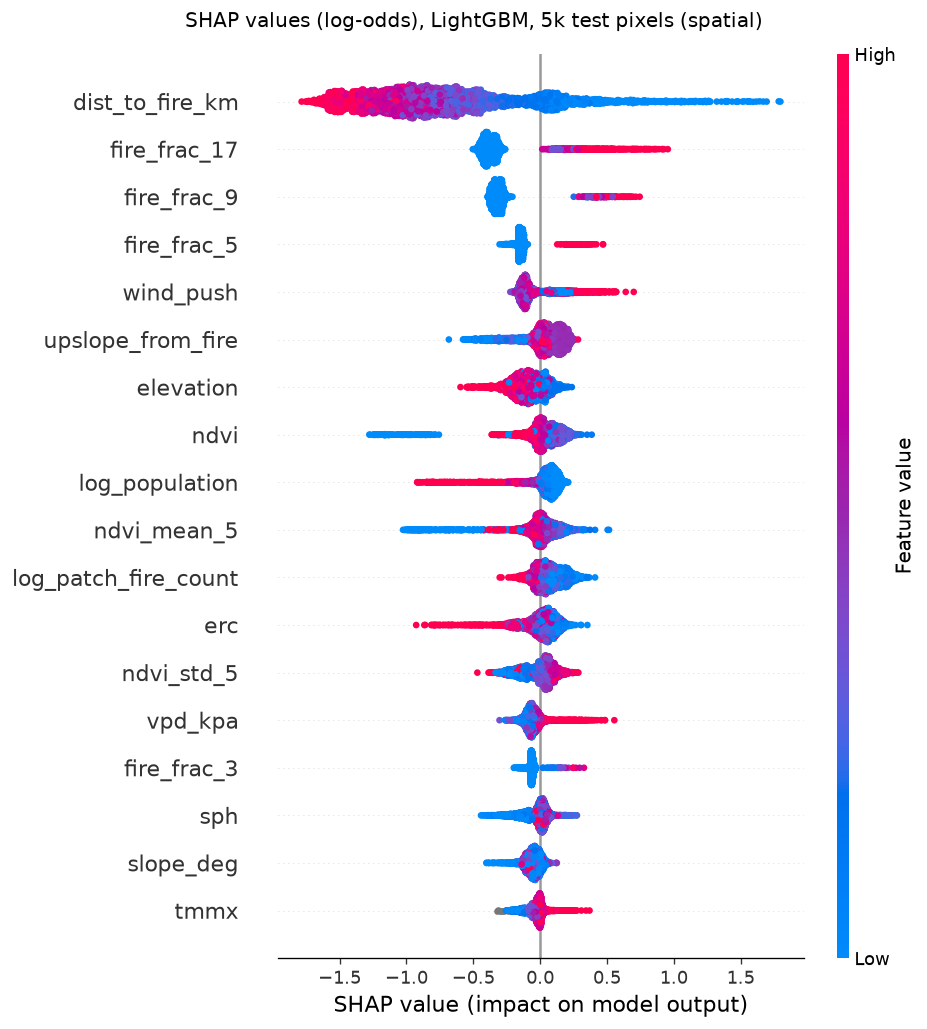
\includegraphics[width=\columnwidth]{results/spatial/shap_summary.png}
\caption{SHAP summary for LightGBM on 5{,}000 spatial-test pixels.}
\label{fig:shap}
\end{figure}

\begin{figure*}[t]
\centering
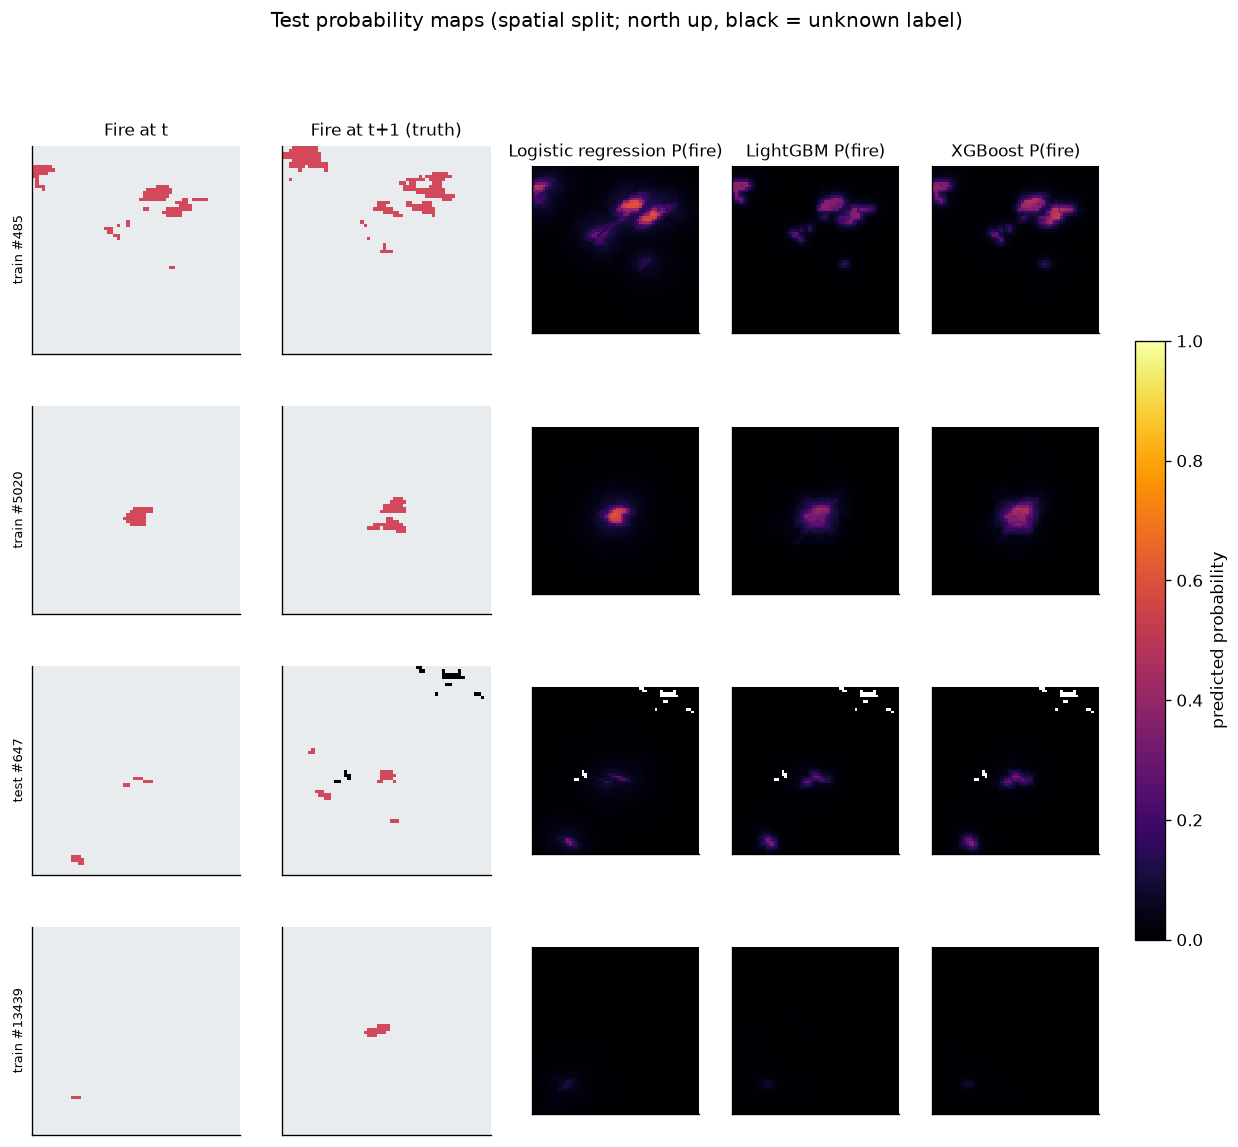
\includegraphics[width=0.9\textwidth]{results/spatial/probability_maps.png}
\caption{Spatial-test examples: fire at $t$, truth at $t{+}1$, and predicted probabilities.}
\label{fig:maps}
\end{figure*}

% -------------------------------------------------------------------------
\section{Discussion and Limitations}
\textbf{Label noise.} MODIS daily detections are affected by clouds and overpass timing, and most next-day fire is new.
This caps achievable precision.
\textbf{Missing drivers.} The data has no fuel moisture, fuel type, suppression or sub-daily wind.
\textbf{Audit coverage.} The terrain fingerprint detects only exact 8$\times$\SI{8}{km} block matches. Partial overlaps
below \SI{64}{km^2} are missed, so the audit gives a lower bound on overlap.
\textbf{Split composition.} The spatial held-out sets contain smaller fires than training, so absolute numbers are
not comparable across protocols. Lift and ROC-AUC are.
\textbf{Phase~2.} A U-Net~\cite{ronneberger2015unet} on the same splits can learn front geometry directly. A hybrid can
feed engineered channels or LightGBM probabilities into the network. It must beat the tuned LightGBM on the spatial
test under a paired test.

\section{Conclusion}
Engineered lagged-burn and wind features with tree ensembles give a strong, reproducible tabular baseline for
next-day spread prediction on NDWS. It exceeds the published tabular baselines and approaches the published CNN.
The official split shares terrain between train and test for about 95\% of test patches, but prevalence-normalised
results and model rankings hold on a location-disjoint split. Patch-bootstrap intervals show that boosting's
advantage over a random forest is not significant. Phase~2 must show that spatial deep models beat this baseline on the
same splits under the same paired test.

\section*{Reproducibility and Contributions}
Code, split manifest and all figures: repository \texttt{fireWild} (\texttt{src/aml}, \texttt{README.md}). Member
contributions are listed in \texttt{CONTRIBUTIONS.md}.

\bibliographystyle{IEEEtran}
\bibliography{references}

\end{document}
